\documentclass[sigplan,nonacm,10pt]{acmart}

\settopmatter{printacmref=false, printccs=false, printfolios=true}
\renewcommand\footnotetextcopyrightpermission[1]{}
\pagestyle{plain}

\usepackage{mathpartir}
\usepackage{stmaryrd}
\usepackage{tikz}
\usetikzlibrary{arrows.meta, positioning, fit, calc}
\usepackage{listings}
\usepackage[capitalize,noabbrev]{cleveref}

\lstdefinelanguage{LeanFour}{
  morekeywords={import,namespace,end,def,theorem,lemma,Prop,Type,let,do,for,in,if,then,else,return,open,section,private,where,match,with},
  sensitive=true,
  morecomment=[l]{--},
  morecomment=[n]{/-}{-/},
  morestring=[b]"
}

\lstset{
  basicstyle=\ttfamily\footnotesize,
  keywordstyle=\bfseries\color{NavyBlue},
  commentstyle=\itshape\color{gray},
  columns=fullflexible,
  keepspaces=true,
  aboveskip=4pt,
  belowskip=4pt
}

\definecolor{NavyBlue}{HTML}{1B365D}
\definecolor{TealInk}{HTML}{2B6CB0}
\definecolor{ForestInk}{HTML}{276749}
\definecolor{AmberInk}{HTML}{B7791F}
\definecolor{TintBlue}{HTML}{EDF4FC}
\definecolor{TintNavy}{HTML}{F4F7FA}
\definecolor{TintAmber}{HTML}{FEFBF3}
\definecolor{TintGreen}{HTML}{F2FBF6}

% Notation macros
\newcommand{\Cinfra}{\mathcal{C}_{\mathrm{infra}}}
\newcommand{\Truth}{\mathcal{E}}
\newcommand{\Orch}{\mathcal{G}}
\newcommand{\Ledger}{\mathcal{L}}
\newcommand{\Events}{\Lambda}
\newcommand{\Spec}{\mathrm{Spec}}
\newcommand{\Prop}{\mathsf{Prop}}
\newcommand{\TypeU}{\mathsf{Type}\;u}
\newcommand{\DefEq}{\equiv_{\beta\delta\iota\zeta}}
\newcommand{\AxiomsZero}{\mathcal{A}_0}
\newcommand{\judge}[3]{#1 \vdash_{\mathrm{accept}} #2 \Downarrow #3}
\newcommand{\irstep}[4]{#1 \xrightarrow{#2}_{#3} #4}
\newcommand{\kw}[1]{\mathsf{#1}}
\newcommand{\code}[1]{\texttt{#1}}
\emergencystretch=1.5em

\title{Proof Irrelevance as a Concurrency Boundary:\\
Decoupling Truth, Verification, and Orchestration in Collaborative Dependent-Type Theorem Proving}

\author{Quod Architecture Working Group}
\affiliation{
  \institution{Quod Project}
  \country{}
}

\begin{abstract}
Collaborative formalization in dependent type theory---specifically Lean~4's Calculus of Inductive Constructions (CIC)---exposes a fundamental tension between concurrent multi-agent search and foundational soundness. Unlike classical first-order reasoning, naive AND-OR proof-search hypergraphs break down under Lean~4's dependent types: splitting an existential construction in $\TypeU$ creates unmergeable witness incompatibilities because $\TypeU$ lacks proof irrelevance, while auxiliary definitions, structures, and typeclass instances cannot be represented as purely propositional edges. Worse, embedding large language models (LLMs) inside the proof orchestrator or verification loop blurs the trusted computing base (TCB).

We present the formal core mechanisms of \textsc{Quod}, an event-sourced, zero-LLM collaborative verification facility for Lean~4. \textsc{Quod} resolves these tensions through three tightly coupled mechanisms:
(1)~an \emph{orthogonal truth--orchestration decoupling} that splits system state into a monotonic, content-addressed \emph{Verified Overlays} truth lattice and a non-monotonic, \code{Route}-grouped task DAG where every worker-facing obligation is a closed $\Prop$ (exploiting CIC proof irrelevance as a concurrency boundary for lock-free racing);
(2)~a \emph{zero-LLM minimal TCB} ($\Cinfra$) enforcing staged verification (static Stage~0 hygiene and minimal-import gates followed by isolated \code{bwrap} Stage~1 Lean~4 kernel definitional-equality and axiom-closure auditing), separation of duties, and kernel-bound credit settlement; and
(3)~a \emph{closed algebraic orchestration IR} (\code{GraphIrOp}) executed over event-sourced finite-state machines across three timescales $(E, C, I)$ with projection-based information-flow isolation.
We formalize the operational semantics of these mechanisms and prove orchestration--soundness non-interference, race-winner irrelevance, kernel-relative soundness, and deterministic event-replay monotonicity.
\end{abstract}

\begin{document}
\maketitle

% =========================================================
\section{Introduction}\label{sec:intro}
% =========================================================

Large-scale formal mathematics increasingly relies on parallel collaboration among human mathematicians and heterogeneous automated provers or LLM coding agents~\cite{demoura2021lean4,mathlib2020}. Yet most agentic theorem-proving frameworks treat the prover harness as a monolith: LLM loops generate tactics, invoke Lean, parse raw compiler errors, rewrite shared files, and maintain ad-hoc proof graphs. When generalized to open, multi-participant settings, this monolithic model suffers from three structural flaws:

\begin{enumerate}
  \item \textbf{Dependent-type splitting hazards.} In Lean~4's Calculus of Inductive Constructions (CIC), proof irrelevance holds for $\Prop$ (\code{Sort 0}) but \emph{not} for computational universes $\TypeU$ (\code{Sort (u+1)}). If a coordinator splits $\exists w : \alpha,\, P(w) \land Q(w)$ into separate constructive subgoals or lets independent workers construct distinct witnesses $w_1 \not\DefEq w_2$, downstream theorems typed against $w_1$ cannot silently consume proofs about $w_2$. Moreover, mathematical developments depend on non-propositional declarations (\code{def}, \code{structure}, \code{instance}, \code{@[simp]}) that cannot be encoded as propositional hypergraph edges.
  \item \textbf{TCB inflation and specification drift.} Placing LLM heuristics or external worker metadata inside the acceptance path risks silent unsoundness via injected \code{axiom}s, \code{sorry}, \code{native\_decide}, metaprogramming (\code{elab}, \code{macro\_rules}), IO backdoors, or specification drift---including vacuous theorem statements.
  \item \textbf{Context pollution and orchestration corruption.} Feeding raw Lean compiler traces to strategic planners degrades reasoning, while allowing untrusted workers to mutate the global task graph invites graph spam and wasted compute.
\end{enumerate}

\textsc{Quod} (\emph{Quod Erat Demonstrandum}) addresses these problems by designing the platform itself as a \emph{zero-LLM deterministic facility} ($\Cinfra$) that strictly separates \emph{mechanism} (soundness, identity, state transitions, and attribution) from \emph{policy} (problem decomposition, market pricing, and proof search).

\paragraph{Motivating Example.}
Throughout this paper we use the \textsc{Quod} Erd\H{o}s Problem~479 specification (\code{examples/\-erdos-479/\-Quod/\-Epoch1/\-Spec.lean}) as a running example:
\begin{lstlisting}[language=LeanFour]
import Mathlib.Data.Int.ModEq
import Mathlib.Data.Set.Finite.Basic
namespace Quod.Epoch1
def erdos_479_stmt : Prop :=
  forall k : Int, k != 1 ->
    { n : Nat | (2 : Int) ^ n == k [ZMOD (n : Int)] }.Infinite
end Quod.Epoch1
\end{lstlisting}
Notice two deliberate invariants already visible in this 11-line specification: (i) the root goal \code{erdos\_479\_stmt} is a closed term of type $\Prop$, and (ii) the specification uses minimal fine-grained imports rather than a blanket \code{import Mathlib}, preventing multi-gigabyte memory thrashing on edge participants and allowing fast isolated kernel audits.

\paragraph{Contributions and Scope.}
We make three core formal contributions grounded directly in the \textsc{Quod} Rust implementation (\code{quod-core}, \code{quod-sandbox}, \code{quod-verifier}, \code{quod-store}, and \code{quod-hub}):
\begin{itemize}
  \item \textbf{Mechanism A (\Cref{sec:mech-a}):} We formalize \textsc{Quod}'s orthogonal decomposition into a monotonic \emph{Verified Overlays} truth layer ($\Truth$) and a non-monotonic \code{Route}-grouped task DAG ($\Orch$) whose worker obligations are uniformly closed $\Prop$ statements. We prove \emph{Orchestration--Soundness Non-Interference} (\Cref{thm:non-interference}) and \emph{Race-Winner Irrelevance} (\Cref{thm:race-irrelevance}).
  \item \textbf{Mechanism B (\Cref{sec:mech-b}):} We formalize the zero-LLM trusted computing base $\Cinfra$ via operational semantics for Stage~0 static hygiene, Stage~1 \code{bwrap}-isolated Lean~4 kernel auditing (\code{isDefEq} + axiom-closure restriction), separation of duties, and atomic credit settlement. We prove \emph{Kernel-Relative Soundness} (\Cref{thm:kernel-soundness}) and \emph{Zero-Self-Report Credit Integrity} (\Cref{thm:credit-integrity}).
  \item \textbf{Mechanism C (\Cref{sec:mech-c}):} We model the closed algebraic orchestration language \code{GraphIrOp} and event-sourced finite-state machines (\code{Epoch}, \code{Task}, \code{Submission}) across three timescales $(E,C,I)$, establishing \emph{Deterministic Event Replay \& Truth Monotonicity} (\Cref{thm:replay}) and \emph{Dependency-Injection Completeness} (\Cref{thm:merge-unlock}).
\end{itemize}
\Cref{sec:impl} maps these semantics to the Rust workspace and explicitly distinguishes implemented core mechanisms from documented architectural extensions (L5 reachability tree-shaking/Git replay and M4 Online-IRT calibration).

% =========================================================
\section{System Model: Three-Timescale $(E, C, I)$ Separation}\label{sec:model}
% =========================================================

\textsc{Quod} structures collaboration along two orthogonal axes: \emph{trust/agency} $(E, C, I)$ and \emph{operational timescale} ($\kw{Scale\;0}$, $\kw{Scale\;1}$, $\kw{Scale\;2}$).

\begin{itemize}
  \item \textbf{Environment / State ($E$):} Persistent mathematical artifacts, task graphs, append-only event logs, and attribution ledgers ($E_0, E_1, E_2$).
  \item \textbf{Deterministic Facility ($C$):} Zero-LLM Rust services and Lean~4 verification sandboxes ($C_0, C_1, C_2$) forming $\Cinfra$. $C$ contains \emph{no} LLM calls, heuristics, or autonomous prompt loops.
  \item \textbf{Isomorphic External Intelligence ($I$):} Human mathematicians and external AI agents acting uniformly as authenticated \code{Actor}s ($I_0$ Workers, $I_1$ Orchestrators, $I_2\text{-B}$ Blueprinters, $I_2\text{-A}$ Auditors).
\end{itemize}

\begin{table}[t]
\centering
\caption{Three-timescale $(E, C, I)$ separation in \textsc{Quod}.}
\label{tab:eci}
\footnotesize
\begin{tabular}{@{}l@{\hspace{5pt}}p{2.05cm}@{\hspace{5pt}}p{2.35cm}@{\hspace{5pt}}p{1.95cm}@{}}
\toprule
\textbf{Scale} & \textbf{State ($E$)} & \textbf{Facility ($C$, 0 LLM)} & \textbf{Actors ($I$)} \\
\midrule
\textbf{Scale 0}\newline{\scriptsize (ms--min)} &
$E_0$: \code{events}, CAS blobs, leases, \code{.olean}, \code{credit\_\-ledger}, Graveyard &
$C_0$: \code{quod-hub} + \code{quod-verifier}, Ed25519 RBAC, Stage~0/1, atomic settlement &
$I_0$ (\code{Worker}): local proof/refutation search, \code{fetch}/\code{submit} \\
\addlinespace
\textbf{Scale 1}\newline{\scriptsize (min--hr)} &
$E_1$: \code{Verified Overlays} + \code{Route}-grouped $\Prop$ DAG + telemetry &
$C_1$: \code{GraphIrOp} validator/interpreter, \code{WakeupDigest}, \code{quod-algo} &
$I_1$ (\code{Orchestrator}): open/prune \code{Route}s, spawn tasks, price bounties \\
\addlinespace
\textbf{Scale 2}\newline{\scriptsize (day--wk)} &
$E_2$: \code{Project} registry, immutable \code{Epoch} \code{Spec}, shared bundles &
$C_2$: minimal-import \& SHA-256 gates, Epoch FSM, (ext: L5 export) &
$I_2\text{-B}$ (\code{Blueprinter}) \& $I_2\text{-A}$ (\code{Auditor}) \\
\bottomrule
\end{tabular}
\end{table}

\paragraph{Isomorphic Authentication and RBAC.}
Every participant (human or agent) registers an Ed25519 public key $pk_a$ bound to an \code{Actor\-Auth\-Context} $(a, \kw{roles}_a, \kw{scopes}_a, \kw{enabled}_a)$ where $\kw{roles}_a \subseteq \{\kw{Worker},\allowbreak \kw{Orchestrator},\allowbreak \kw{Blueprinter},\allowbreak \kw{Auditor},\allowbreak \kw{Admin}\}$. Every mutating HTTP request $(m, p, \tau, b)$ carries headers $(a, \tau, \sigma)$ verified inside $C_0$ against the canonical signing payload:
\begin{multline*}
\kw{payload}(m, p, \tau, b) = \kw{upper}(m) \,\|\, \text{\code{"\textbackslash n"}} \,\|\, p \\
  \,\|\, \text{\code{"\textbackslash n"}} \,\|\, \tau \,\|\, \text{\code{"\textbackslash n"}} \,\|\, \kw{SHA256}(b),
\end{multline*}
enforcing bounded clock skew $|\tau_{\mathrm{now}} - \tau| \le \Delta_{\max}$, role membership, and project scope containment ($\kw{scopes}_a = \emptyset$ denotes global scope; otherwise $pid \in \kw{scopes}_a$). Delegation is strictly stratified: \code{Blueprinter}s may issue invite tokens only for \code{Worker} or \code{Orchestrator} within their own \code{project\_scopes}, whereas \code{Auditor}, \code{Admin}, and unscoped invites require \code{Admin} authority.

\begin{figure}[t]
\centering
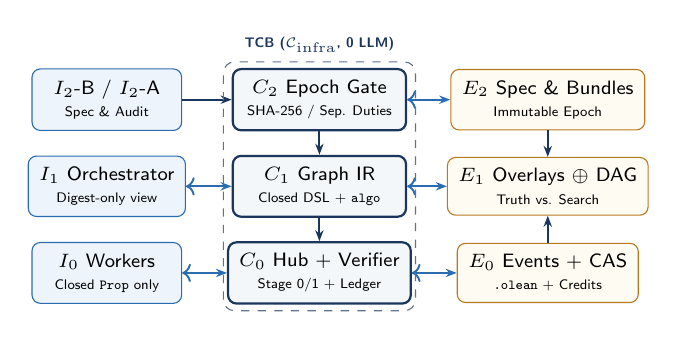
\begin{tikzpicture}[
  x=1cm, y=1cm,
  boxI/.style={rectangle, rounded corners=3pt, draw=TealInk, fill=TintBlue, font=\sffamily\scriptsize, align=center, inner sep=4pt, minimum width=1.9cm, minimum height=0.72cm},
  boxC/.style={rectangle, rounded corners=3pt, draw=NavyBlue, thick, fill=TintNavy, font=\sffamily\scriptsize, align=center, inner sep=4pt, minimum width=2.2cm, minimum height=0.72cm},
  boxE/.style={rectangle, rounded corners=3pt, draw=AmberInk, fill=TintAmber, font=\sffamily\scriptsize, align=center, inner sep=4pt, minimum width=2.1cm, minimum height=0.72cm},
  arr/.style={-{Stealth[length=4pt]}, line width=0.7pt, draw=NavyBlue},
  darr/.style={<-{Stealth[length=4pt]}, line width=0.7pt, draw=TealInk}
]
\node[boxI] (I2) at (0, 2.2) {$I_2$-B / $I_2$-A\\{\tiny Spec \& Audit}};
\node[boxC] (C2) at (2.7, 2.2) {$C_2$ Epoch Gate\\{\tiny SHA-256 / Sep. Duties}};
\node[boxE] (E2) at (5.6, 2.2) {$E_2$ Spec \& Bundles\\{\tiny Immutable Epoch}};

\node[boxI] (I1) at (0, 1.1) {$I_1$ Orchestrator\\{\tiny Digest-only view}};
\node[boxC] (C1) at (2.7, 1.1) {$C_1$ Graph IR\\{\tiny Closed DSL + \code{algo}}};
\node[boxE] (E1) at (5.6, 1.1) {$E_1$ Overlays $\oplus$ DAG\\{\tiny Truth vs. Search}};

\node[boxI] (I0) at (0, 0.0) {$I_0$ Workers\\{\tiny Closed \code{Prop} only}};
\node[boxC] (C0) at (2.7, 0.0) {$C_0$ Hub + Verifier\\{\tiny Stage 0/1 + Ledger}};
\node[boxE] (E0) at (5.6, 0.0) {$E_0$ Events + CAS\\{\tiny \code{.olean} + Credits}};

\draw[arr] (I2) -- (C2);
\draw[darr] (C2) -- (E2);
\draw[darr] (I1) -- (C1);
\draw[darr] (C1) -- (E1);
\draw[darr] (I0) -- (C0);
\draw[darr] (C0) -- (E0);

\draw[arr] (C2) -- (C1);
\draw[arr] (C1) -- (C0);
\draw[arr] (E0) -- (E1);
\draw[arr] (E2) -- (E1);

\draw[dashed, NavyBlue!70, rounded corners=4pt] (1.48, -0.48) rectangle (3.92, 2.68);
\node[anchor=south, font=\sffamily\tiny\bfseries, text=NavyBlue] at (2.7, 2.68) {TCB ($\Cinfra$, 0 LLM)};
\end{tikzpicture}
\caption{Authority flow and TCB boundary across $(E, C, I)$ and the three operational timescales.}
\Description{Three-by-three grid showing I, C, E across Scales 0, 1, and 2, with C forming the Zero-LLM TCB.}
\label{fig:eci}
\end{figure}

% =========================================================
\section{Mechanism A: Orthogonal Truth--Orchestration Decoupling}\label{sec:mech-a}
% =========================================================

We now formalize why splitting $E_1$ into an append-only truth layer and a mutable orchestration layer—coupled with the restriction that every worker task is a closed $\Prop$—makes concurrent proof search sound by construction.

\subsection{Why Naive Hypergraphs Fail in CIC}
Consider a constructive existential specification $\exists w : \alpha,\, P(w) \land Q(w)$. In a naive AND-OR hypergraph that decomposes this goal into two parallel worker tasks ``construct $w_1 : \alpha$ with $P(w_1)$'' and ``construct $w_2 : \alpha$ with $Q(w_2)$'', the soundness of merging depends on $w_1 \DefEq w_2$, which fails whenever workers choose distinct witnesses. Similarly, splitting $P(w)$ and $Q(w)$ across a shared definition $w : \alpha$ requires introducing a non-propositional \code{def} into the Lean environment before either lemma typechecks. Thus, \emph{truth accumulation} (extending a Lean \code{Environment}) and \emph{proof-search orchestration} (proposing, prioritizing, and pruning subgoals) are fundamentally different algebraic objects.

\subsection{Dual-Layer State Decomposition}

\begin{definition}[Monotonic Truth Layer $\Truth$]\label{def:truth-layer}
For a project $pid$ and active epoch $e$, the truth layer (\emph{Verified Overlays}) is a finite partial map $\Truth : \kw{ModName} \rightharpoonup \kw{OverlayEntry}$ where each entry $(k, \kw{src}, \kw{olean}, h, \kw{imps})$ consists of an overlay kind $k \in \{\kw{Spec}, \kw{DefOverlay}, \kw{ProvedTask}\}$, source UTF-8 text $\kw{src}$, compiled binary $\kw{olean}$, content hash $h = \kw{SHA256}(\kw{src})$, and declared imports $\kw{imps} \subseteq \mathrm{dom}(\Truth)$. $\Truth$ is ordered by monotonic extension:
\begin{multline*}
\Truth \sqsubseteq \Truth' \iff \mathrm{dom}(\Truth) \subseteq \mathrm{dom}(\Truth') \\
  \land \forall m \in \mathrm{dom}(\Truth),\, \Truth'(m) = \Truth(m).
\end{multline*}
Furthermore, every module $m \in \mathrm{dom}(\Truth)$ must compile cleanly in Lean~4 against its declared imports $\kw{imps}$ with zero \code{sorry} and axioms restricted to $\AxiomsZero$.
\end{definition}

\begin{definition}[Non-Monotonic Orchestration Layer $\Orch$]\label{def:orch-layer}
The orchestration layer is a \code{Route}-grouped directed acyclic graph $\Orch = (R, V, D_{\mathrm{dep}}, D_{\mathrm{ref}})$:
\begin{itemize}
  \item $R$ is a finite map of exploration routes $r \mapsto (\kw{title}, \kw{state}_r)$ with $\kw{state}_r \in \{\kw{Active},\allowbreak \kw{Won},\allowbreak \kw{Pruned},\allowbreak \kw{Refuted}\}$.
  \item $V$ is a finite map of task nodes $v \mapsto (\rho_v, \phi_v, I_v, s_v, \beta_v)$, where:
    \begin{itemize}
      \item $\rho_v \in \{\kw{Root},\allowbreak \kw{Lemma},\allowbreak \kw{Connector},\allowbreak \kw{Merge},\allowbreak \kw{Refutation},\allowbreak \kw{AuxLemma},\allowbreak \kw{WitnessBundle},\allowbreak \kw{Porting}\}$ is the tactical role;
      \item $\phi_v$ is a \emph{closed} target proposition such that $\Truth \vdash \phi_v : \Prop$ (either referencing a locked declaration or an inline $\Prop$ term);
      \item $I_v \subseteq \mathrm{dom}(\Truth)$ is the node's \code{curated\_\-imports};
      \item $s_v \in \kw{TaskState}$ is the lifecycle state; and $\beta_v = (\kw{prio}_v, p_v, c_v, k_v, \kw{tier}_v, b_v)$ holds scheduling and bounty parameters.
    \end{itemize}
  \item $D_{\mathrm{dep}} \subseteq V \times V$ are \code{DependsOn} edges (maintained acyclic) and $D_{\mathrm{ref}} \subseteq V \times V$ are \code{Refutes} edges.
\end{itemize}
\end{definition}

Unlike $\Truth$, $\Orch$ is \emph{non-monotonic}: routes may be pruned, priorities and bounties patched, and subgoals reorganized without ever retracting or mutating entries in $\Truth$.

\subsection{The Closed-$\Prop$ Uniformity Protocol}
Every task claimable by an external worker $I_0$ is uniformly a closed $\Prop$ obligation. \Cref{tab:closed-prop} summarizes how diverse collaborative proving patterns reduce to closed $\Prop$ tasks in \textsc{Quod}.

\begin{table}[t]
\centering
\caption{Uniform encoding of collaborative semantics as closed $\Prop$ tasks.}
\label{tab:closed-prop}
\footnotesize
\begin{tabular}{@{}p{2.7cm}@{\hspace{6pt}}p{5.0cm}@{}}
\toprule
\textbf{Collaboration Pattern} & \textbf{Closed $\Prop$ Encoding in $\Orch$} \\
\midrule
Direct subgoal lemma & Target $\phi_v \equiv G : \Prop$ (\code{Lemma}, \code{AuxLemma}) \\
Counterexample probe & Target $\phi_v \equiv \neg P : \Prop$ (\code{Refutation}) \\
Pre-split sufficiency check & Target $\phi_v \equiv P_1 \to P_2 \to G : \Prop$ (\code{Connector}) \\
Cross-route equivalence bridge & Target $\phi_v \equiv A \to B : \Prop$ (\code{Lemma}) \\
Existential witness coupling & $\kw{Nonempty}\; B : \Prop$ (\code{WitnessBundle}), or derive $h_{\mathrm{ex}} : \exists w,\, \mathrm{Spec}\; w$ and decouple via \code{Classical.choose} \\
Post-hoc composition & Target $\phi_v \equiv G : \Prop$ with $\kw{depends\_on} = [P_1, P_2]$; $C_0$ auto-injects proved overlays into $I_v$ (\code{Merge}) \\
\bottomrule
\end{tabular}
\end{table}

\paragraph{The Privileged \code{DefOverlay} Channel.}
When downstream propositions must \code{unfold} a concrete definition $f : \alpha \to \beta$ in $\TypeU$ rather than quantifying over an abstract witness, $I_1$ or $I_2$ submits a pure-definition module via \code{PublishDefOverlay(\-module\_name,\; code)}. Once compiled with zero \code{sorry} and checked across every constant in \code{modData.constNames} against $\AxiomsZero$, it enters $\Truth$ as an immutable \code{OverlayKind::\-DefOverlay}. Subsequent worker tasks simply import that module in $I_v$ while remaining 100\% closed $\Prop$ obligations.

\paragraph{Anti-Wasted-Work Safeguards.}
Two protocol mechanisms prevent workers from proving useless subgoals: (i) for an expensive split of $G$ into $P_1, P_2$, $I_1$ spawns a low-cost \code{Connector} task $P_1 \to P_2 \to G$ concurrently to validate sufficiency early; (ii) \code{quod-algo::check\_coupling} flags sibling open tasks in the same \code{Route} whose statements contain $\exists$, \code{Exists}, or \code{Nonempty}, alerting $I_1$ to bundle coupled witnesses via \code{WitnessBundle} or \code{DefOverlay}.

\subsection{Metatheory: Proof Irrelevance as a Concurrency Boundary}

Let $\mathcal{M}_{\mathrm{Lean}}(\Truth)$ denote the Lean~4 kernel typing judgment under the verified environment formed by $\Truth$. We write $\Truth \models_{\mathrm{core}} \phi$ if there exists a closed proof term $t$ in $\Truth$ with $\Truth \vdash t : \phi$ and axioms in $\AxiomsZero$.

\begin{theorem}[Orchestration--Soundness Non-Interference]\label{thm:non-interference}
For any sequence of valid system transitions $\Sigma_0 \to \Sigma_1 \to \dots \to \Sigma_n$ under arbitrary adversarial or buggy actions by $I_1$ (orchestrator) and $I_0$ (workers):
\begin{enumerate}
  \item Every entry $m \in \mathrm{dom}(\Truth_n)$ of kind \code{ProvedTask} for task $v$ witnesses $\Truth_n \models_{\mathrm{core}} \phi_v$;
  \item If project status reaches $\kw{Proved}$ on root task $v_{\mathrm{root}}$ (whose $\phi_{v_{\mathrm{root}}}$ equals the audited epoch specification $\phi_{\Spec}$), then $\Truth_n \models_{\mathrm{core}} \phi_{\Spec}$;
  \item No sequence of \code{GraphIrOp} actions by $I_1$ (creating/pruning routes, reprioritizing, mispricing bounties, or injecting false priors) can cause an unproved proposition to satisfy $\Truth_n \models_{\mathrm{core}} \phi_{\Spec}$.
\end{enumerate}
\end{theorem}

\begin{proof}
By structural induction on the transition trace $\Sigma_0 \to^* \Sigma_n$.
\emph{Base case:} $\Sigma_0$ contains only the audited \code{Spec} module $m_{\Spec}$, which defines $\phi_{\Spec} : \Prop$ without proving it.
\emph{Inductive step:} Transitions modifying $\Orch$ (\code{GraphIrOp} except \code{PublishDefOverlay}) leave $\Truth$ unchanged ($\Truth_{i+1} = \Truth_i$). Transitions modifying $\Truth$ occur exclusively via \code{record\_verification\_outcome} inside $\Cinfra$ after Stage~0 and Stage~1 kernel acceptance (\Cref{sec:mech-b}). By Stage~1 auditing (\code{AuditHarness}), a \code{Proof} submission for task $v$ is inserted into $\Truth_{i+1}$ only if candidate declaration $d$ compiles in $\Truth_i$ with $\mathrm{collectAxioms}(d) \subseteq \AxiomsZero$ and $\kw{isDefEq}\;\mathrm{type}(d)\;\phi_v$. Since $\Truth_i \sqsubseteq \Truth_{i+1}$ is monotonic, all previously valid derivations remain valid in $\Truth_{i+1}$. Finally, \code{project\_proved} is set iff a verified \code{Proof} completes $v_{\mathrm{root}}$ or a \code{Merge} task whose non-inline declaration name matches $\kw{spec\_decl\_name}$ (\code{memory.rs:2271--2287}), yielding $\Truth_n \models_{\mathrm{core}} \phi_{\Spec}$.
\end{proof}

\begin{theorem}[Race-Winner Irrelevance]\label{thm:race-irrelevance}
Suppose $k \ge 2$ concurrent $I_0$ workers submit distinct valid proofs $c_1, c_2$ for the same open task $v$ with closed target $\phi_v : \Prop$ importing $I_v \subseteq \mathrm{dom}(\Truth)$. Regardless of which submission wins \emph{First-Verified-Valid Wins}, the set of propositions provable in any downstream module importing $m_v$ is invariant.
\end{theorem}

\begin{proof}
Because $\phi_v : \Prop$ is closed and Stage~1 checks $\mathrm{type}(d_j) \DefEq \phi_v$ for both candidates $j \in \{1, 2\}$, both candidate declarations $d_1, d_2$ expose definitionally identical types $\phi_v : \Prop$ (and both only export the audited target interface or closed lemmas over $I_v$). By proof irrelevance in CIC, any two inhabitants $d_1, d_2 : \phi_v$ are definitionally equal ($d_1 \DefEq d_2 : \phi_v$). Moreover, downstream tasks import $m_v$ solely as an opaque verified module to prove closed $\Prop$ statements (or unfold concrete definitions fixed deterministically in prior \code{DefOverlay}s). Hence replacing $d_1$ by $d_2$ preserves well-typedness and provability of all downstream tasks in $\Orch$.
\end{proof}

Notice how \Cref{thm:race-irrelevance} fails if worker tasks could return arbitrary witnesses in $\TypeU$: \emph{Proof Irrelevance} in CIC is precisely what makes lock-free competitive racing over $\Prop$ tasks safe!

% =========================================================
\section{Mechanism B: Zero-LLM Minimal TCB \& Staged Verification Semantics}\label{sec:mech-b}
% =========================================================

To maintain LCF-style trustworthiness~\cite{gordon1979edinburgh}, \textsc{Quod} bounds its trusted computing base strictly to $\Cinfra$:
\begin{multline*}
\mathrm{TCB} = \{\text{Lean 4 kernel},\; \text{Stage 0 gate},\; \text{\code{bwrap}/cgroup},\\
  \text{\code{AuditHarness}},\; \text{Rust FSM/Store}\}.
\end{multline*}
External agents $I$, model lineage tags, worker local \code{quod verify} claims, and client-reported scores are untrusted inputs.

\subsection{Operational Semantics of Staged Verification}
Let a submission be $\sigma = (\kw{id}, a, v, \kappa, m_c, d_c, \kw{code}, I_c)$ with actor $a$, task $v$, kind $\kappa \in \{\kw{Proof}, \kw{Refutation}, \kw{DefOverlay}\}$, candidate module $m_c$, declaration $d_c$, source $\kw{code}$, and imports $I_c$. Let $\mathcal{P}_0 = (\kw{max\_bytes}, \mathcal{F}_{\mathrm{tok}}, h_{\Spec}^{\star})$ be \code{Stage0Policy}, where in \code{quod-sandbox/src/lib.rs}:
\begin{small}
\begin{align*}
\kw{max\_bytes} &= 262{,}144, \\
\mathcal{F}_{\mathrm{tok}} &= \{\code{axiom}, \code{opaque}, \code{unsafe}, \code{implemented\_by}, \\
&\qquad \code{extern}, \code{native\_decide}, \code{sorry}, \code{admit}, \code{\#eval}, \\
&\qquad \code{\#print}, \code{\#check}, \code{elab}, \code{macro\_rules}, \code{IO.}, \code{System.}\}, \\
\AxiomsZero &= \{\code{propext},\allowbreak \code{Classical.choice},\allowbreak \code{Quot.sound}\}.
\end{align*}
\end{small}
Additionally, \code{check\_\-spec\_\-minimal\_\-imports} rejects any specification line (after stripping \code{--} comments) equal to \code{import Mathlib}.

\begin{figure*}[t]
\centering
\begin{minipage}{\textwidth}
\small
\begin{mathpar}
\inferrule*[right=\textsc{S0-Ok}]
{
  |\kw{code}| \le 262{,}144 \\
  h_{\Spec} = h_{\Spec}^{\star} \\
  \forall t \in \mathcal{F}_{\mathrm{tok}},\, \neg\kw{HasToken}(\kw{code}, t)
}
{
  \mathcal{P}_0 \vdash_{\mathrm{S0}} (\kw{code}, h_{\Spec}) \Downarrow \kw{Ok}(\kw{SHA256}(\kw{code}))
}
\and
\inferrule*[right=\textsc{S1-Proof}]
{
  \kw{bwrap}(\Truth, I_c, \kw{code}) \Downarrow \kw{Compiled}(E) \\
  E.\kw{find}(d_c) = \kw{Some}(ci) \\
  \kw{collectAxioms}(E, d_c) \subseteq \AxiomsZero \\
  E \vdash ci.\kw{type} \DefEq \phi_v
}
{
  \Truth \vdash_{\mathrm{S1}} (\kw{Proof}, m_c, d_c, \kw{code}, I_c, \phi_v) \Downarrow \kw{Valid}(\kw{olean})
}
\and
\inferrule*[right=\textsc{S1-Refute}]
{
  \kw{bwrap}(\Truth, I_c, \kw{code}) \Downarrow \kw{Compiled}(E) \\
  E.\kw{find}(d_c) = \kw{Some}(ci) \\
  \kw{collectAxioms}(E, d_c) \subseteq \AxiomsZero \\
  E \vdash ci.\kw{type} \DefEq (\neg \phi_v)
}
{
  \Truth \vdash_{\mathrm{S1}} (\kw{Refutation}, m_c, d_c, \kw{code}, I_c, \phi_v) \Downarrow \kw{Valid}(\bot)
}
\and
\inferrule*[right=\textsc{S1-DefOverlay}]
{
  \kw{bwrap}(\Truth, I_c, \kw{code}) \Downarrow \kw{Compiled}(E) \\
  C = E.\kw{moduleConsts}(m_c) \neq \emptyset \\
  \forall c \in C,\, \kw{collectAxioms}(E, c) \subseteq \AxiomsZero
}
{
  \Truth \vdash_{\mathrm{S1}} (\kw{DefOverlay}, m_c, \kw{code}, I_c) \Downarrow \kw{Valid}(\kw{olean})
}
\and
\inferrule*[right=\textsc{Accept-FirstWins}]
{
  s_v \in \{\kw{Open}, \kw{Racing}, \kw{StalledSoft}\} \\
  \mathcal{P}_0 \vdash_{\mathrm{S0}} (\kw{code}, h_{\Spec}) \Downarrow \kw{Ok}(h) \\
  \Truth \vdash_{\mathrm{S1}} (\kw{Proof}, \dots) \Downarrow \kw{Valid}(\kw{olean}) \\
  \Truth' = \Truth[m_c \mapsto \kw{entry}] \quad
  \Orch' = \Orch[v \mapsto \kw{Proved}] \quad
  \Ledger' = \Ledger \mathbin{\Vert} (a, v, \kw{bounty}(v))
}
{
  (\Truth, \Orch, \Ledger, \Events) \vdash_{\mathrm{commit}} (\sigma, v) \Downarrow (\Truth', \Orch', \Ledger', \Events')
}
\and
\inferrule*[right=\textsc{Reject-RaceLost}]
{
  s_v \in \{\kw{Proved}, \kw{RefutedHard}, \kw{Pruned}, \kw{StaleEpoch}\} \\
  \Truth \vdash_{\mathrm{S1}} (\kappa, \dots) \Downarrow \kw{Valid}(\_)
}
{
  (\Truth, \Orch, \Ledger, \Events) \vdash_{\mathrm{commit}} (\sigma, v) \Downarrow
  (\Truth,\; \Orch,\; \Ledger,\; \Events \mathbin{\Vert} \kw{RaceLost}(\sigma.\kw{id}))
}
\and
\inferrule*[right=\textsc{Epoch-Audit}]
{
  e.\kw{state} = \kw{PendingAudit} \\
  e.\kw{created\_by} \neq a \\
  \kw{Auditor} \in \kw{roles}_a \\
  \kw{MinimalImports}(e.\kw{spec})
}
{
  e \xrightarrow{\kw{ApproveAudit}(a)} e[\kw{state} \mapsto \kw{Active}, \kw{audited\_by} \mapsto a]
}
\end{mathpar}
\end{minipage}
\caption{Operational rules of $\Cinfra$: Stage~0 static policy, Stage~1 \code{bwrap} + Lean~4 kernel auditing, atomic first-verified-valid-wins settlement, and Epoch separation of duties.}
\Description{Inference rules S0-Ok, S1-Proof, S1-Refute, S1-DefOverlay, Accept-FirstWins, Reject-RaceLost, and Epoch-Audit.}
\label{fig:verification-rules}
\end{figure*}

\Cref{fig:verification-rules} specifies the core acceptance judgments. Stage~1 executes inside an unprivileged Linux namespace sandbox (\code{BwrapRunner}) mounting the shared read-only \code{toolchain\_bundle} and epoch-isolated \code{accepted\_\-olean/\-<project\_id>/\-epoch\_<E>/}, under cgroup~v2 memory and CPU time caps. Notice that \code{AuditHarness} emits \code{QUOD\_AUDIT\_JSON:\{"ok":true\}} only if the Lean~4 metaprogram completes without throwing any audit error.

\paragraph{Anti-Triviality Reduction Checking.}
For reduction-style checks (\code{peelReduction} in \code{lean-harness/\-Audit\-Harness.\-lean.\-tmpl}), the harness traverses nested $\forall$-binders $e \equiv \forall (x_1 : d_1) \cdots (x_k : d_k),\, \phi_{\mathrm{rem}}$ until $\phi_{\mathrm{rem}} \DefEq \phi_{\Spec}$ and rejects:
\begin{itemize}
  \item empty reductions ($k = 0$, \code{QUOD\_\-AUDIT\_\-TRIVIAL\_\-EMPTY\_\-REDUCTION});
  \item non-propositional binders ($\neg\kw{isProp}(d_i)$, \code{QUOD\_\-AUDIT\_\-NON\_\-PROP\_\-SUBGOAL});
  \item dependent subgoals ($d_i.\kw{hasFVar}$, \code{QUOD\_\-AUDIT\_\-DEPENDENT\_\-SUBGOAL}); and
  \item trivial subgoals ($d_i \DefEq \bot$ or $d_i \DefEq \phi_{\Spec}$).
\end{itemize}

\begin{theorem}[Kernel-Relative Soundness]\label{thm:kernel-soundness}
Assuming soundness of the Lean~4 kernel and OS namespace/filesystem isolation of \code{bwrap}, if $\judge{(\Truth,\Orch,\Ledger,\Events)}{\sigma}{(\Truth',\Orch',\Ledger',\Events')}$ adds $(m_c, \kw{entry})$ to $\Truth'$ for task $v$ with kind \code{Proof} (resp.\ \code{Refutation}), then $\Truth' \models_{\mathrm{core}} \phi_v$ (resp.\ $\Truth' \models_{\mathrm{core}} \neg\phi_v$) using at most $\AxiomsZero$.
\end{theorem}

\begin{proof}
Acceptance requires both \textsc{S0-Ok} and \textsc{S1-Proof} (or \textsc{S1-Refute}). \textsc{S0-Ok} verifies specification hash equality $h_{\Spec} = h_{\Spec}^{\star}$ and excludes all token-level escape hatches in $\mathcal{F}_{\mathrm{tok}}$ (\code{sorry}, \code{axiom}, \code{native\_decide}, \code{elab}, \code{IO.}, etc.). Stage~1 executes \code{lean} inside \code{bwrap} with read-only base toolchains and isolated per-epoch \code{.olean}s, preventing ambient file tampering. Inside the rendered \code{AuditHarness}, \code{collectAxioms} checks the full transitive axiom closure of $d_c$ against $\AxiomsZero$, and \code{isDefEq} checks definitional equality against $\phi_v$ (or \code{Not} applied to $\phi_v$). Only upon exit status~0 and \code{QUOD\_AUDIT\_JSON:\{"ok":true\}} does \textsc{Accept-FirstWins} persist the \code{.olean} and extend $\Truth$.
\end{proof}

\begin{theorem}[Zero-Self-Report Credit Integrity]\label{thm:credit-integrity}
Every entry $(a, v, pts)$ appended to \code{credit\_ledger} ($\Ledger$) corresponds bijectively to a unique \textsc{Accept-FirstWins} transition for a non-terminal task $v$ whose winning submission passed Stage~0 and Stage~1 verification inside $\Cinfra$.
\end{theorem}

\begin{proof}
Inspecting the hub API and store interface (\code{quod-store}), no external endpoint accepts credit amounts or self-reported verification verdicts. The sole mutating path appending to $\Ledger$ and emitting \code{CreditAwarded} is \code{record\_\-verification\_\-outcome} (\code{memory.rs:2160--2194}) invoked by the trusted \code{quod-verifier} daemon when $\kw{verdict.ok} = \kw{true}$, $\kappa \in \{\kw{Proof}, \kw{Refutation}\}$, and $s_v$ was not yet terminal. Any competing valid submission arriving afterward hits \textsc{Reject-RaceLost} and awards zero points.
\end{proof}

% =========================================================
\section{Mechanism C: Closed Algebraic Orchestration IR \& Event-Sourced Effect Isolation}\label{sec:mech-c}
% =========================================================

Whereas $I_0$ workers speak Lean~4 code, $I_1$ orchestrators mutate $\Orch$ exclusively through a closed, strongly-typed algebraic command language, preventing arbitrary script execution inside $C_1$.

\subsection{The Closed Algebraic Command DSL (\code{GraphIrOp})}
An orchestration transaction is an atomic batch $\kw{ApplyIrRequest} = (\kw{ops}, \kw{dry\_run})$ where each operation $op \in \kw{GraphIrOp}$ (\code{crates/\-quod-core/\-src/\-ir.rs}) belongs to an 8-constructor sum type:
\begin{small}
\begin{align*}
op ::= &\ \kw{CreateRoute}(rid, \kw{title}, \kw{rationale}) \\
\mid &\ \kw{PruneRoute}(rid, \kw{reason}) \\
\mid &\ \kw{SpawnTask}(tid, rid?, \rho, \kw{decl}, \phi, \kw{inline}, d_c, I_v, \kw{deps}, \kw{ref}?, \beta) \\
\mid &\ \kw{LinkDependency}(v_{\mathrm{up}}, v_{\mathrm{down}}) \\
\mid &\ \kw{PublishDefOverlay}(m, \kw{code}) \\
\mid &\ \kw{SetDispatchPolicy}(\kw{algo}, \epsilon, \kw{cross\_route}) \\
\mid &\ \kw{PatchNodeBudget}(tid, \beta') \\
\mid &\ \kw{PatchActorHint}(a, \kw{tier}?, \kw{tags}?, \kw{enabled}?)
\end{align*}
\end{small}
Here $\kw{algo} \in \{\kw{WeightedVoi},\allowbreak \kw{LineageDiversity},\allowbreak \kw{TierMatched},\allowbreak \kw{PriorityQueue}\}$ is a closed enumeration of $C_0$ dispatch algorithms. Crucially:
\begin{enumerate}
  \item \code{ApplyIrRequest} is validated and applied \emph{atomically} (supporting \code{dry\_run} validation without state mutation);
  \item \code{PatchActorHint} with \code{enabled = false} writes only to per-project \code{project\_\-actor\_\-blocks}, never globally banning shared workers across projects; and
  \item \code{PublishDefOverlay} does not insert directly into $\Truth$---it enqueues a sandboxed \code{VerificationJob} of kind \code{DefOverlay}, returning its \code{overlay\_\-job\_\-ids} for kernel verification.
\end{enumerate}

\subsection{Event-Sourced Finite-State Machines}
Every state mutation emits an append-only event into $\Events$ alongside materialized projections (\Cref{fig:fsms}). In \code{crates/\-quod-core/\-src/\-fsm.rs}:
\begin{itemize}
  \item \textbf{\code{EpochState}:} $\kw{PendingAudit} \to \{\kw{Active}, \kw{Archived}\}$; $\kw{Active} \to \kw{Freezing} \to \kw{Migrating} \to \kw{Archived}$.
  \item \textbf{\code{TaskState}:} $\kw{Blocked} \xrightarrow{\kw{UnblockDeps}} \kw{Open} \xrightarrow{\kw{AcquireLease}} \kw{Racing} \xrightarrow{\kw{AllExpired}} \kw{StalledSoft}$; any dispatchable state transitions via \code{AcceptProof} to \code{Proved}, or via \code{HardRefuted} / \code{Prune} / \code{FreezeEpoch} to terminal \code{RefutedHard} / \code{Pruned} / \code{StaleEpoch} (\code{StaleEpoch} may migrate to \code{Open} in a new epoch).
  \item \textbf{\code{SubmissionState}:} $\kw{SealedReceived} \to \kw{Stage0SpecOk} \to \kw{Stage1KernelOk} \to \kw{Stage2HygieneOk} \to \{\kw{Merged},\allowbreak \kw{RejectedRaceLost}\}$, with explicit typed rejection states for spec drift, security, kernel failure, hygiene, resource limits, and stale epochs.
\end{itemize}

\begin{figure}[t]
\centering
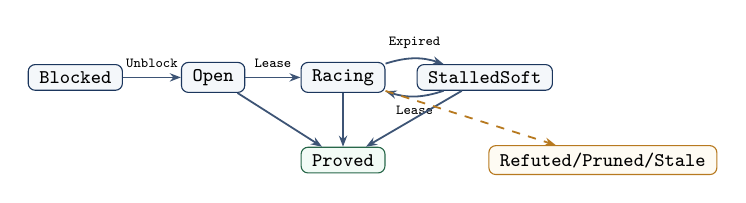
\begin{tikzpicture}[
  x=1cm, y=1cm,
  st/.style={rectangle, rounded corners=2.5pt, draw=NavyBlue, fill=TintNavy, font=\sffamily\scriptsize, inner xsep=4pt, inner ysep=2.5pt},
  term/.style={rectangle, rounded corners=2.5pt, draw=ForestInk, fill=TintGreen, font=\sffamily\scriptsize\bfseries, inner xsep=4pt, inner ysep=2.5pt},
  arr/.style={-{Stealth[length=4pt]}, line width=0.65pt, draw=NavyBlue!85}
]
\node[st] (B) at (0, 0) {\code{Blocked}};
\node[st] (O) at (1.75, 0) {\code{Open}};
\node[st] (R) at (3.4, 0) {\code{Racing}};
\node[st] (S) at (5.2, 0) {\code{StalledSoft}};
\node[term] (P) at (3.4, -1.05) {\code{Proved}};
\node[st, draw=AmberInk, fill=TintAmber] (T) at (6.7, -1.05) {\code{Refuted/Pruned/Stale}};

\draw[arr] (B) -- node[above, font=\tiny] {\code{Unblock}} (O);
\draw[arr] (O) -- node[above, font=\tiny] {\code{Lease}} (R);
\draw[arr] (R) to[bend left=18] node[above, font=\tiny] {\code{Expired}} (S);
\draw[arr] (S) to[bend left=18] node[below, font=\tiny] {\code{Lease}} (R);
\draw[arr] (O) -- (P);
\draw[arr] (R) -- (P);
\draw[arr] (S) -- (P);
\draw[arr, dashed, draw=AmberInk] (R) -- (T);
\end{tikzpicture}
\caption{Core \code{TaskState} transition graph enforced in \code{quod-core::fsm}.}
\Description{Directed graph of TaskState transitions from Blocked to Open, Racing, StalledSoft, Proved, and terminal states.}
\label{fig:fsms}
\end{figure}

\subsection{Auto-Injection, Unblocking, and Information-Flow Isolation}
When a \code{Proof} submission for upstream task $u$ passes Stage~1 and merges into $\Truth$ as module $m_u$, $C_0$ atomically propagates dependencies across every edge $(u, w) \in D_{\mathrm{dep}}$:
\begin{enumerate}
  \item $I_w \leftarrow I_w \cup \{m_u\}$ (injecting the verified overlay into $w$'s \code{curated\_imports});
  \item if $\forall u' \in \kw{deps}(w),\, s_{u'} = \kw{Proved}$ and $s_w = \kw{Blocked}$, transition $s_w$ via \code{UnblockDependencies} to \code{Open} and emit \code{TaskUnlocked}.
\end{enumerate}

\paragraph{Information-Flow Projections.}
To prevent context pollution across timescales, $C_1$ exposes a lossy, compiler-noise-free projection
\[
\pi_{\mathrm{digest}} : (\Truth, \Orch, \Events) \to \kw{WakeupDigest}
\]
containing only route summaries, blocked/open/stalled counts, top-\code{VOI} candidates, and stall alerts. Raw Lean compiler error stacks are routed to $E_0$'s \code{Graveyard} for $I_0$ workers retrying the same task, never dumped into $I_1$'s strategic context. Complementarily, $C_1$ provides stateless pure functions in \code{quod-algo}: \code{voi\_rank} (scoring $(1-p)\cdot\kw{prio}\cdot(1+0.5\cdot\kw{unblocks})/c$), \code{detect\_stalls} (cross-lineage failure counts $\ge 2$, failed attempts $\ge 4$, or timeouts $\ge 2$), \code{check\_coupling}, and \code{mine\_reusable\_overlays}. Similarly, $I_2\text{-A}$ (Auditor) operates in an isolated context from $I_2\text{-B}$ (Blueprinter) to detect vacuous truth in specifications.

\subsection{Metatheory of Event-Sourced Orchestration}

\begin{theorem}[Deterministic Event Replay \& Truth Monotonicity]\label{thm:replay}
Let $\Events = [e_1, \dots, e_k]$ be the append-only event log generated by valid \code{GraphIrOp} and verification transitions starting from $\Sigma_0$. Materialized projection replay $\llbracket \Events \rrbracket(\Sigma_0)$ is deterministic, and for all prefixes $\Events_1 \preceq \Events_2$ within an epoch, $\Truth(\Events_1) \sqsubseteq \Truth(\Events_2)$.
\end{theorem}

\begin{proof}
Every FSM transition (\code{EpochState::\-transition}, \code{TaskState::\-transition}, \code{SubmissionState::\-transition}) is a deterministic total/partial function over algebraic enums, and \code{ApplyIrRequest} applies \code{GraphIrOp} constructors deterministically in list order. In $\Truth$, only \code{DefOverlayVerified} and \code{Proof} acceptance insert new keys $(pid, e, m)$ into \code{overlays}; no transition deletes or overwrites an existing verified overlay within an epoch. Hence $\Truth(\Events_1) \sqsubseteq \Truth(\Events_2)$ holds for all prefixes.
\end{proof}

\begin{theorem}[Dependency-Injection Completeness for Merge Tasks]\label{thm:merge-unlock}
Whenever a \code{Merge} task $w$ transitions from \code{Blocked} to \code{Open} via \code{UnblockDependencies}, every upstream prerequisite module $\{m_u \mid (u, w) \in D_{\mathrm{dep}}\}$ already resides in $\Truth$ and is present in $w$'s \code{curated\_imports} $I_w$.
\end{theorem}

\begin{proof}
Because $D_{\mathrm{dep}}$ is acyclic and each upstream task $u$ transitions to \code{Proved} at most once (\Cref{fig:fsms}, \code{Proved} is terminal), the transition of $u$ atomically executes \code{record\_\-verification\_\-outcome} (\code{memory.rs:2202--2251}), which inserts $m_u$ into $\Truth$, appends $m_u$ to $I_w$ for all downstream $w$, and only fires \code{Unblock\-Dependencies} once \code{all\_\-dependencies\_\-proved} evaluates to \code{true}. Thus at unlock time, all upstream overlays are both verified in $\Truth$ and imported by $w$.
\end{proof}

% =========================================================
\section{Implementation \& Architectural Extensions}\label{sec:impl}
% =========================================================

The mechanisms formalized in \Cref{sec:mech-a,sec:mech-b,sec:mech-c} are implemented across six Rust crates: \code{quod-core} (RBAC, FSMs, \code{GraphIrOp}, \code{quod-algo}, evaluator traits), \code{quod-store} (PostgreSQL~16 using runtime \code{sqlx::query} for offline buildability plus an in-memory store and content-addressed blob store), \code{quod-sandbox} (Stage~0, minimal-import check, \code{AuditHarness} rendering, \code{BwrapRunner}), \code{quod-verifier} (bounded concurrent verification daemon), \code{quod-hub} (Axum REST API, \code{/JOIN.md}, \code{/skills/*}, and public portal), and \code{quod-cli} (single static binary embedding role skills). Projects share read-only \code{toolchain\_bundles} (e.g., 7.4\,GB Mathlib4 \code{v4.36.0}) via \code{bwrap} while isolating per-project \code{accepted\_olean/<project\_id>/epoch\_<E>/}.

\paragraph{Anti-Stampede Dispatch and Bounty Economics.}
$C_0$ supports dual-mode task claiming: explicit task selection by bounty/tier or automated matching via \code{WeightedVoi}, \code{LineageDiversity}, \code{TierMatched}, or \code{PriorityQueue}, bounded by per-task \code{racer\_cap\_k}, cross-lineage diversity scoring, and per-actor active lease limits. Unspecified bounties default deterministically via \code{compute\_\-default\_\-bounty(\-expected\_cost\_c,\; priority,\; failed\_attempts)} in $[10, 5000]$.

\paragraph{Documented Architectural Extensions.}
Two components specified in \code{docs/architecture.md} extend this core as roadmap modules rather than completed runtime services:
(i)~\textbf{L5 Tree-Shaking \& Prefix-Buildable Git Export} (\code{quod export}), whose Lean~4 transitive dependency walker skeleton exists in \code{lean-harness/\-SliceExtractor.lean} to prune dead routes via backward constant reachability and replay winning overlays in topological order into a clean, contributor-attributed Git repository; and
(ii)~\textbf{M4 \code{quod-evaluator}}, a planned stateless service replaying \code{events} and \code{Canary} anchors to calibrate Online-IRT / Bradley--Terry difficulty and actor skill parameters from unbiased \code{propensity\_\-score} telemetry (currently abstracted behind the \code{Capability\-Evaluator} trait in \code{quod-core::\-evaluator}).

% =========================================================
\section{Related Work \& Conclusion}\label{sec:related}
% =========================================================

\paragraph{Small-Kernel Verification and Collaborative Lean.}
LCF~\cite{gordon1979edinburgh} established the principle of isolating a tiny trusted kernel behind an extensible tactic layer; Lean~4~\cite{demoura2021lean4} continues this tradition with an independent type-checking kernel and \code{collectAxioms} auditing. Large-scale collaborative formalizations over Mathlib~\cite{mathlib2020} rely heavily on human-curated \code{leanblueprint} dependency graphs~\cite{massot2024blueprint}, which visually organize informal-to-formal decompositions but lack automated Stage~0/1 multi-agent sandboxing, closed $\Prop$ racing boundaries, and event-sourced bounty markets.

\paragraph{Agentic Proving and Trusted Infrastructure.}
Recent LLM theorem-proving agents couple search heuristics tightly with Lean compilation inside a single harness. \textsc{Quod} inverts this architecture: by removing all LLMs from $\Cinfra$, splitting truth ($\Truth$) from orchestration ($\Orch$), and enforcing closed $\Prop$ tasks via staged kernel audits, \textsc{Quod} enables open, heterogeneous human--AI swarms to collaborate concurrently without ever sacrificing foundational soundness.

\begin{thebibliography}{4}

\bibitem{demoura2021lean4}
Leonardo de Moura and Sebastian Ullrich.
\newblock 2021.
\newblock The Lean 4 Theorem Prover and Programming Language.
\newblock In \emph{Automated Deduction -- CADE 28} (LNCS, Vol. 12699). Springer, 625--635.

\bibitem{gordon1979edinburgh}
Michael J.~C. Gordon, Robin Milner, and Christopher P. Wadsworth.
\newblock 1979.
\newblock \emph{Edinburgh LCF: A Mechanised Logic of Computation}.
\newblock Lecture Notes in Computer Science, Vol. 78. Springer.

\bibitem{mathlib2020}
The mathlib Community.
\newblock 2020.
\newblock The Lean Mathematical Library.
\newblock In \emph{Proceedings of the 9th ACM SIGPLAN International Conference on Certified Programs and Proofs (CPP '20)}. ACM, 367--381.

\bibitem{massot2024blueprint}
Patrick Massot.
\newblock 2024.
\newblock Lean Blueprint: Formalization Planning and Dependency Visualization for Lean 4.
\newblock Software and documentation, \url{https://github.com/PatrickMassot/leanblueprint}.

\end{thebibliography}

\end{document}
